\chapter{Background}

\section{vroom}
Vroom is a userspace NVMe driver written in Rust. As of this writing, it offers high performance and the functionality required for general I/O operations, but it is not yet production-ready. Unlike interrupt-driven drivers, vroom uses polling to determine the state of the I/O operations. Polling is often preferable in high-performance applications, as interrupts are relatively performance-intensive operations \cite{spdksubmitting}.
When using vroom without the IOMMU, the BAR of the NVMe is exposed in the pseudo-filesystem \texttt{sysfs} e.g., for the device with PCI address \texttt{0000:01:00.0} under the path \texttt{/sys/bus/PCI/devices/0000:01:00.0/resource0}. Direct memory access is performed using physical addresses on hugepages.

An NVMe driver consists of submission and completion queues implemented as ring buffers. The driver adds commands to the submission queue, which the NVMe controller reads and executes. The executed command gets placed on a corresponding completion queue. A deeper explanation of the steps will be provided in \autoref{c:impl}.
As vroom does not have a kernel driver part, we unbind the kernel driver and bind it to Pci-stub. Pci-stub is a dummy driver that occupies the PCI driver such that the kernel or another application cannot bind to the device.

\section{Memory Management Unit}
% weird writing, not clear
Memory Management Units (MMU) for the CPU have been used since the 1980s. After their first integrated application featuring on Intel's 80286 chip \cite{intel80286}, they have since become the de facto standard for addressing computer memory. By providing processes with a virtual address space instead of physical addresses, every process is isolated and only has access to memory assigned to it virtual address space. Each translated address points to a region of memory called a page. These pages can have different sizes, with the default being \qty{4}{\kibi\byte} pages on modern x86-64 architectures.

The translations of these pages are stored in so-called page tables. As one page table does not offer enough address space, multiple tables are linked together, consisting of pointers to a lower-level page table. Each table stores parts of the address, and the entry can be determined by using the offset. One page table walk thus includes fetching multiple tables from memory, resulting in a high latency. To circumvent this, a Translation Lookaside Buffer (TLB) is used to cache translations.

The TLB is very performant to access. Frequent access to the same address can be done at a fraction of the time needed for a page table walk. A TLB miss describes the scenario in which a physical address needs to be translated, but it has no entry in the TLB, resulting in an expensive page walk.

\section{I/O Memory Management Unit}
The advantages and success of the CPU's MMU and the introduction of the PCIe bus specification have incentivized hardware manufacturers to apply this concept to peripheral device buses. In 2006, Intel introduced their "Virtualization Technology for Directed I/O" (Intel VT-d) and AMD their "AMD I/O Virtualization Technology" (AMD-Vi/IOMMU). In this thesis, the term IOMMU references both technologies. The IOMMU was originally only used for "solving the addressing problems of devices with limited address space" \cite{vfiokerneldocs}, but nowadays is used mainly for virtualization and device isolation.

The IOMMU works similarly to the MMU, but instead of mapping memory to a process's virtual address space, it maps it to an I/O virtual address space for device access. The addresses used are called I/O Virtual Addresses (IOVA).
On a 4-level page table structure as the IOMMU uses for \qty{4}{\kibi\byte} pages, one address resolution results in 4 memory accesses.

The IOMMU, like the MMU has a TLB, which is called the I/O Translation Lookaside Buffer (IOTLB). The size of the IOTLB is not officially documented by Intel nor AMD \cite{iommuhuber}.

\begin{figure}[H]
    \centering
    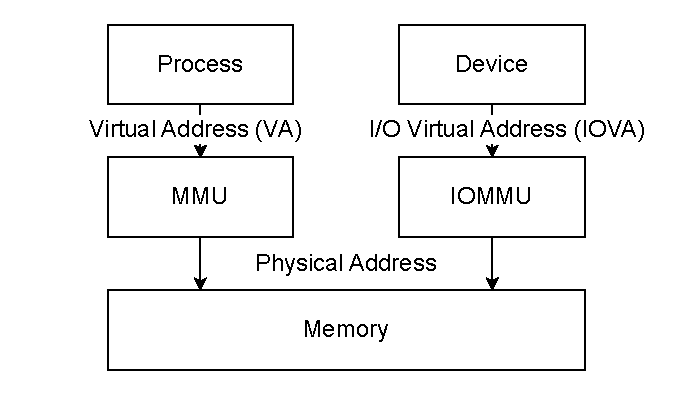
\includegraphics[width=0.6\textwidth]{figures/MMUIOMMU.pdf}
    \caption{MMU and IOMMU relation to physical memory, adapted from \cite{iommuscalability}}
    \label{fig:mmuvsiommu}
\end{figure}

The IOMMU paging structures of Intel's VT-d consist of \qty{4}{\kibi\byte} page tables storing 512 8-byte entries. The IOMMU uses the upper portions to determine the location of the stored page tables and the lower portion of the address as page offset. In the case of \qty{4}{\kibi\byte} pages its 12 bits, for \qty{2}{\mebi\byte} its 21.


% todo maybe add amd-v figure

% \begin{figure}[H]
%     \centering
%     \subcaptionbox {Translation of a \qty{4}{\kibi\byte} page} {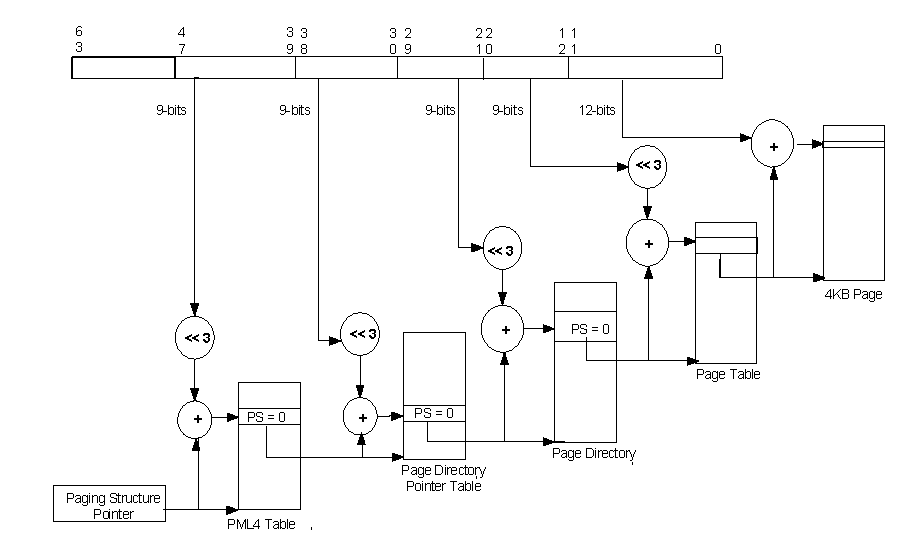
\includegraphics[width=0.9\textwidth]{figures/4kibtranslation.pdf}\label{fig:pagewalk4kib}}
%     \subcaptionbox {Translation of a \qty{2}{\mebi\byte} page} {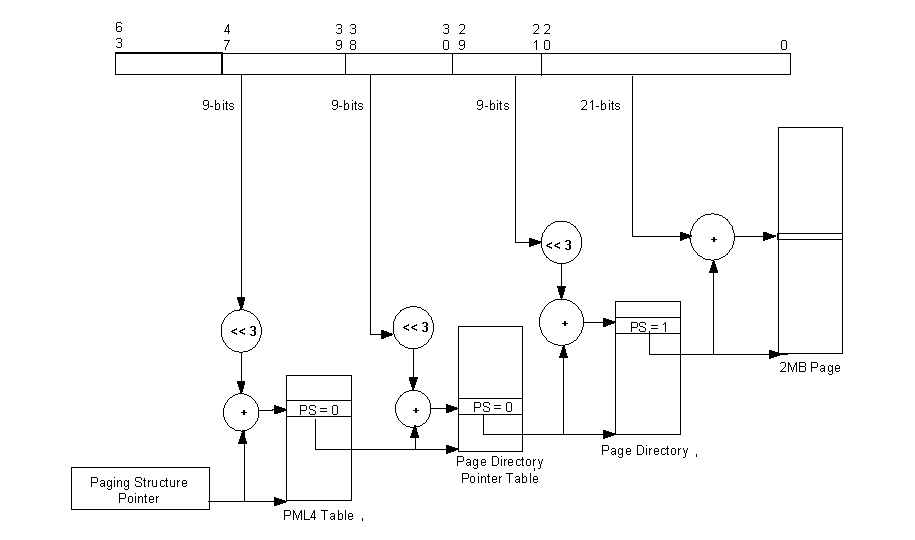
\includegraphics[width=0.9\textwidth]{figures/2mibtranslation.pdf}\label{fig:pagewalk2mib}}
%     \caption{Intel VT-d Paging structure for translating a 48-bit address to a \qty{4}{\kibi\byte} and a \qty{2}{\mebi\byte} page, grabbed from \cite{vtdspec}}
%     \label{fig:pagewalk}
% \end{figure}

\begin{figure}[H]
    \centering
    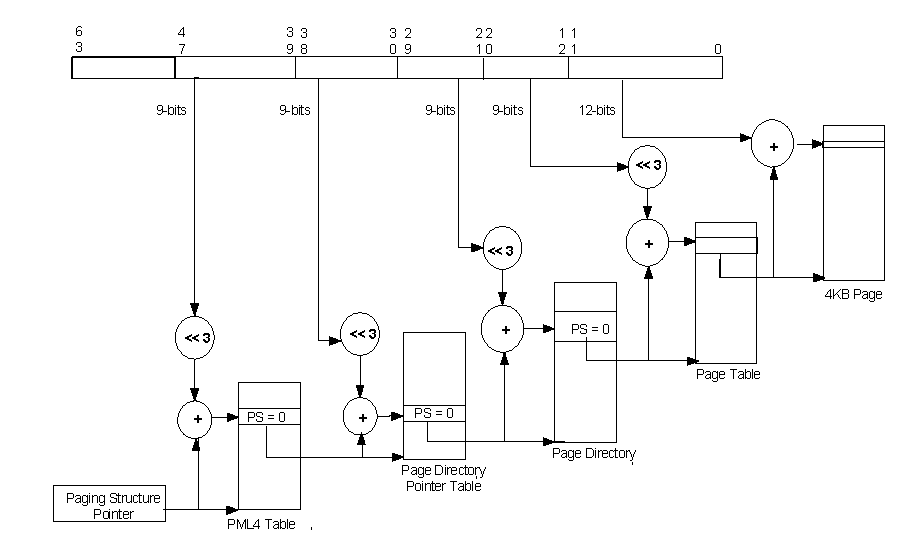
\includegraphics[width=0.9\textwidth]{figures/4kibtranslation.pdf}
    \caption{Intel VT-d Paging structure for translating a 48-bit address to a \qty{4}{\kibi\byte} page, grabbed from \cite{vtdspec}}
    \label{fig:pagewalk}
\end{figure}

% \section{Memory Mapped I/O}
% Memory Mapped I/O, in contrast to Port-Mapped I/O, places devices in the same address space as the main memory. Instead of using Assembly instructions like \texttt{in} or \texttt{out}, a device can be addressed just like the RAM can be. Addressing this memory itself can currently be done in two ways. Either accessing it with the physical address or using a hardware translation device like the I/O Memory Management Unit (IOMMU). Before our implementation, vroom only supported the former.

\section{Direct Memory Access}
Using Direct Memory Access, we can bypass the CPU for I/O operations. Previously, this was handled by a separate DMA-controller hardware (third-party DMA), but using PCI, we can directly access it through bus mastering (first-party DMA) \cite{maellmann}. Using the IOMMU, the request is intercepted and translated to the physical address.

\section{Hugepages}
As the demand for bigger memory mappings, e.g., for big files, increased, the amount of TLB cache misses rose proportionally. With modern CPUs TLB typically having space for only 4096 \qty{4}{\kibi\byte} pages, only an address space of \qty{16}{\mebi\byte} could be stored and accessed quickly \cite{emmerich2019user}. To increase the virtual memory space, hardware producers reacted by providing bigger page sizes on their architectures than the default \qty{4}{\kibi\byte}.
Linux currently provides two ways of using Hugepages.
In the optimal case, using a \qty{2}{\mebi\byte} or \qty{1}{\gibi\byte} page size should result in a 512- or 262144-times reduction in cache misses compared to \qty{4}{\kibi\byte} pages. This makes a huge difference, especially in high-performance computing.

\begin{itemize}
    \item \textbf{Persistent Hugepages}: Persistent Hugepages are reserved in the kernel and cannot be swapped or used for another purpose. These hugepages can be mounted as a (pseudo) filesystem called \texttt{hugetlbfs}, which can be mounted to a directory. The amount and size of the pages can be specified either during boot on the kernel command line with, e.g., \texttt{hugepagesz=1g hugepages=16} or dynamically using the Linux \texttt{proc} virtual filesystem \cite{hugetlbkerneldocs}.
    \item \textbf{Transparent Hugepages}: Transparent Hugepages are a more recent addition to the kernel. Transparent hugepages are not fixed or reserved in the kernel and allow all unused memory to be used for other purposes. THPs provide a way of utilizing the TLB effectively without reserving vast amounts of memory. The \texttt{khugepaged} daemon scans memory and collapses sequences of basic pages into bigger pages. THPs can either be enabled, disabled, or only be used on \texttt{madvise(MADV\_HUGEPAGE)} memory regions \cite{transhugekerneldocs}.
\end{itemize}

Vroom currently uses hugepages for DMA and locks them with the Linux syscall \texttt{mlock} to prevent the kernel from swapping them out.
Hugepages have to be used to prevent the kernel from moving data from one physical page to another physical page. The kernel cannot move these pages like \qty{4}{\kibi\byte} pages. This is called 'page pinning'. Other userspace drivers like SPDK or DPDK also rely on this to perform DMA without the IOMMU.

\section{Peripheral Component Interconnect Express}
PCIe is a standard for peripheral device buses. Each device on the PCI bus has a unique PCI address, segmented into three parts, as seen in \autoref{fig:pciaddress}. The maximum data payload size of PCIe is \qty{4}{\kibi\byte}.

\begin{figure}[H]
    \centering
    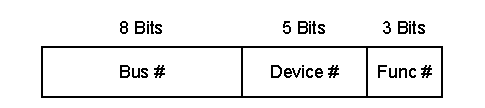
\includegraphics[width=.7\textwidth]{figures/pciaddress.pdf}
    \caption{Segmented PCI identifier}
    \label{fig:pciaddress}
\end{figure}

Each device on the bus uses a PCIe configuration space, which includes registers for controlling the device's behavior, e.g., enabling DMA in the command register. It also includes Base Address Registers (BAR), which are used to access the device's actual controller. The configuration space can be seen on \autoref{fig:pciconfig}. The marked fields are needed for Vroom.

\begin{figure}[H]
    \centering
    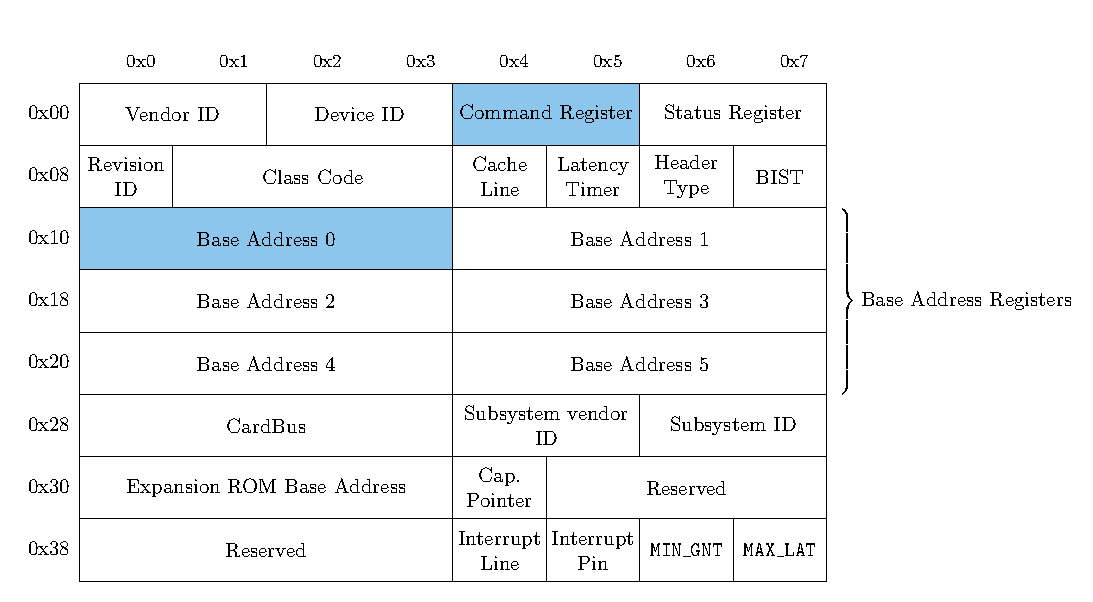
\includegraphics[width=\textwidth]{figures/pcie-config-space}
    \caption{PCIe configuration space, adapted from \cite{vroom}}
    \label{fig:pciconfig}
\end{figure}

% % maybe remove 
% \section{Character and Block Devices}
% Unix/Linux uses two types of devices: Character and Block devices. Character devices are used for devices with small amounts of data and no frequent seek queries, like keyboard and mouse.
% Block devices typically have large data volumes and are organized in blocks, like HDDs and SSDs.
% Read and Write operations on character devices are done sequentially byte-by-byte, while on block devices, read/write is done at the data block level.
% These constraints also impact how the drivers for these devices work. CDev drivers directly communicate with the device drivers, while block device drivers work in conjunction with the kernel file management and block device subsystem. This allows efficient asynchronous read/write operations for large data amounts, but small byte-sized data transfer achieves lower latency on character devices.

% % maybe remove 
% \section{Non-Uniform Memory Access}
% Non-Uniform Memory Access is a type of system architecture for multi-CPU systems. Hardware resources are bundled into "nodes". These nodes can contain multiple CPUs, memory, and I/O buses \cite{numakerneldocs}. This can relieve stress on the memory bus and improve performance if the memory is part of the same node as the CPU. On the other hand, performance may decrease if the memory is situated in another node. With \texttt{numactl}, it is possible to specify the locality of memory and CPU to run a process on one node \cite{numactlmanpage}.

\section{Rust}
While userspace drivers can theoretically and practically be written in any language, as proven by the network driver Ixy \cite{ixylanggithub}, Rust excels as it not only offers memory safety but memory safety without garbage collection. This is especially important, as garbage-collected languages have overhead and latency spikes, which can lower performance. Another critical factor is that, like C, Rust does not use exceptions. Being forced to handle errors ensures no rogue exception can take down critical code infrastructure.
Additionally, Rust provides low-level access while offering a high-level development experience through zero-cost abstractions.